\chapter{Probabilidade}
\inic Neste capítulo, abordaremos os conceitos fundamentais da teoria das probabilidades, que constituem a base para o entendimento da inferência estatística. Em particular, na parte matemática, haverá momentos de maior rigor teórico. De modo geral, a probabilidade é amplamente aplicável em diversas áreas do conhecimento, tanto em pesquisas quantitativas quanto qualitativas. O objetivo deste capítulo é apresentar a probabilidade em nível de graduação, com ênfase em situações-problema relacionadas às áreas mencionadas no capítulo anterior.


\section{Histórico}
\inic A primeira manifestação foi dada por meio de jogos de dados, mas não é um dado qualquer era o conhecido como astrágalo, pequeno osso do tarso, situado entre a tíbia e o calcâneo. Este era usado como uma espécie de ``dado".

    \begin{figure}[h]
    \caption{Ástragalo}
		\centering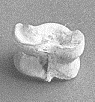
\includegraphics[scale=1]{figuras/astralagos}
	\end{figure}
	
\inic Usava-se o astrágalo para: previsão do futuro, divisão de heranças e disputas esportivas. As pesquisa na área de probabilidade iniciaram com Edmond Halley (1656 - 1665) e Girolamo Cardano (1570), quando estes estavam preocupados em fazer estimativas de taxas de seguro de vida. Depois disso, muito da teoria rigorosa foi desenvolvida pela família Bernoulli, mais especificamente com Daniel Bernoulli.

\section{Experimentos Aleatório}
\begin{defin}[Experimento aleatórios]
São aqueles que ao serem repetidos nas mesmas condições não produzem os mesmos resultados.
\end{defin}
\exemplo 
\begin{enumerate}
		\item[(i)] Retiradas de peças em um lote de peças numa fábrica, verificar quais são defeituosas;
		\item[(ii)] Escolher uma pessoa em um estádio de futebol para participar da partida;
		\item[(iii)] Verificar quantas toneladas de lixo foram depositados em um determinado local;
		\item [(iv)] Lançar um dado e verificar qual a face que se encontra voltada para cima;
		\item [(v)] Verificar se em um determinado dia choverá ou não.
	\end{enumerate}
Não são experimentos aleatórios
	\begin{enumerate}
		\item[(i)] Lançar uma pedra para o cima e verificar o que acontece;
		\item[(ii)] Dar partida num carro e verificar a distância percorrida após 10 segundos.
	\end{enumerate}
\inic Estaremos interessados em experimentos aleatórios, onde predomina a incerteza. 
\section{Espaço Amostral}
\begin{defin}[Espaço Amostral]
Denominamos espaço amostral associado a um experimento $\varepsilon$ o conjunto $\mathnormal{S}$ ou $\mathnormal{\Omega}$ de seus possíveis resultados.
\end{defin}
Isto é, listamos todos os possíveis resultados de um experimento aleatório temos o espaço amostral.

\exemplo
\begin{enumerate}
		\item[(i)] Lançamento de um dado possui espaço amostral $\mathnormal{\Omega} = \{1,2,3,4,5,6\}$;
		\item[(ii)]  Em uma moeda, represente $\mathnormal{K}$ o número de coroas e $\mathnormal{C}$ o número de cara. Verifica-se a face que caiu para cima, o espaço amostral é $\mathnormal{\Omega} = \{\mathnormal{C},\mathnormal{K}\}$;
		\item[(iii)] Sejam as condições do item (ii), suponha duas moedas, o espaço amostral é
		$$\mathnormal{\Omega} = \{\mathnormal{CC,CK,KC,KK}\}$$
		\item[(iv)] Três peças são retiradas de uma linha de produção. Cada peça é classificada como boa ($\mathnormal{B}$) ou defeituosa ($\mathnormal{D}$), o espaço amostral associado a esse experimento é dado por 
		$$\mathnormal{S} = \{\mathnormal{BBB, BBD, BDB,\dots, DDB, DDD}\}$$
		\item[(v)] Uma moeda é lançada até aparecer a primeira vez cara, o espaço amostral é
			$$\mathnormal{\Omega} = \{\mathnormal{C, KC, KKC, KKKC},\dots\}.$$
		\item [(vi)] Quantidade de pessoas que entram em uma determinada loja.
		\item [(vii)] Número de animais que existem em uma determinada região;
	\end{enumerate}
\inic Note que o espaço amostral dos itens (v) e (vi) são espaços de cardinalidade ($|\Omega|$) infinita, porém contável, pois não possui uma quantidade máxima de possíveis lançamentos e é possível enumerar estes elementos. Um espaço amostral que será muito útil é o do lançamento de dois dados, que é descrito por

\begin{equation}
\label{EAU}
	\mathnormal{\Omega}=\left[
	\begin{array}{cccccc}
	(1,1) & (1,2) & (1,3)& (1,4)&(1,5)&(1,6)\\
	(2,1) & (2,2) & (2,3)& (2,4)&(2,5)&(2,6)\\
	(3,1) & (3,2) & (3,3)& (3,4)&(3,5)&(3,6)\\
	(4,1) & (4,2) & (4,3)& (4,4)&(4,5)&(4,6)\\
	(5,1) & (5,2) & (5,3)& (5,4)&(5,5)&(5,6)\\
	(6,1) & (6,2) & (6,3)& (6,4)&(6,5)&(6,6)\\
	\end{array}
	\right]
\end{equation}
\begin{defin}[Evento]
 Chamamos de evento a todo resultado ou subconjunto de resultados de um experimento.
\end{defin}

\exemplo
\begin{enumerate}
	\item[(i)] No experimento de retirada de peças de um lote, seja o evento $\mathnormal{E}$: Retirar duas peças boas, o conjunto $\mathnormal{E}$ é dado por $\mathnormal{E}=\{\mathnormal{BBD}, \mathnormal{BDB}, \mathnormal{DBB}\}$;
	\item[(ii)] Considere o experimento lançar a moeda até dar cara, e defina os evento $\mathnormal{E}_1$: Dar cara no lançamento múltiplo de 2. Temos os conjuntos $\mathnormal{E}_1 = \{\mathnormal{KC,KKKC, KKKKKC,} \dots \}$;
	\item[(iii)] Escolhe-se um animal de um determinada região dada, temos o evento: ``o animal é uma felino".
	\item [(iv)] Em um conjunto de pessoas, escolhe-se uma ao acaso, e temos o evento: ``A pessoa é mulher"
\end{enumerate}
\inic Nosso objetivo é modelar os eventos e comparar com o espaço amostral. Calcular probabilidades é medir um fato aleatório e descrevermos qual destes é mais provável de ocorrer tal atitude ajuda a na tomada de decisões.

\subsection{Operações com Eventos}
\begin{enumerate}
	\item [(i)] A reunião de dois eventos $\mathnormal{A}$ e $\mathnormal{B}$, denotada por $\mathnormal{A \cup B}$ é o evento que ocorre se pelo menos um deles ocorre; 
	
	\begin{figure}[H]
    \caption{União de dois eventos}
		\centering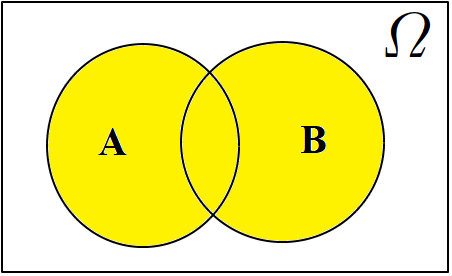
\includegraphics[scale=1]{figuras/uniao}
	\end{figure}
	
	\item [(ii)] A interseção de dois eventos $\mathnormal{A}$ e $\mathnormal{B}$, denotada por $\mathnormal{A} \cap \mathnormal{B}$, é o evento que ocorre quando ambos ocorrem;
	
	\begin{figure}[H]
    \caption{União de dois eventos}
		\centering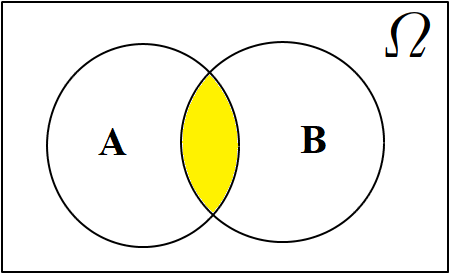
\includegraphics[scale=1]{figuras/inter}
	\end{figure}
	
	\item [(iii)] O complementar de um evento $\mathnormal{A}$, denotado por $\mathnormal{A}^c$ ou $\mathnormal{\overline{A}}$ é o evento que ocorre quando $\mathnormal{A}$ não ocorre.
	\begin{figure}[H]
            \caption{Evento Complementar}
		\centering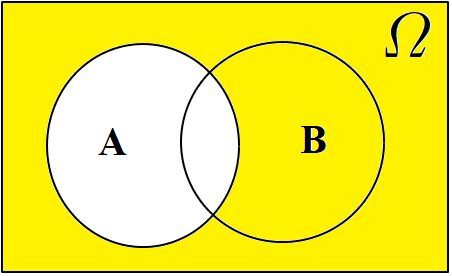
\includegraphics[scale=1]{figuras/comp.png}
	\end{figure}
\end{enumerate}
\inic Note que para (iii) a interseção não está em $A^c$ apesar de estar em $B$. Outra observação importante é que se $A\cap B = \phi$ então chamamos $A$ e $B$ de mutuamente exclusivos, isto é, eventos que não podem ocorrer juntos. Agora apresentaremos o Lema \ref{lema1} que pode ser muito útil quando se fala em manipulações com conjuntos. 

\begin{lema}
\label{lema1} Sejam $\mathnormal{A,B}$ e $\mathnormal{C}$ eventos de um espaço amostral $\mathnormal{\Omega}$, são válidas as relações
    \begin{enumerate}
		\item[(i)] $(\mathnormal{A\cup B})\cap \mathnormal{C} = (\mathnormal{A\cap C})\cup (\mathnormal{B \cap C})$;
		\item[(ii)] $\mathnormal{(A\cap B)\cup C = (A\cup C)\cap (B \cup C)}$;
		\item[(iii)] $\mathnormal{(A \cup B)^c = A^c \cap B^c}$;
		\item[(iv)] $\mathnormal{(A \cap B)^c = A^c \cup B^c}$.
	\end{enumerate}
\end{lema}
\inic A demonstração do Lema \ref{lema1} é facilmente encontrada em \cite{magalhaes2006probabilidade}, e também pode ser notada na forma dos diagramas de Veen. Faremos agora uma breve análise ``filosófica" a respeito do conceito de probabilidade esta que tem diversas abordagens. 

\section{Probabilidade Subjetiva}
\inic É a probabilidade que é baseada na crença do observador.
	\begin{enumerate}
		\item[(i)] Qual a probabilidade de chover hoje às 17:00?
		\item[(ii)] Qual a probabilidade de um clube ganhar todos os jogos da temporada?
		\item[(iii)] Qual a probabilidade de uma mulher grávida parir em um ambulância verde, no estado de Goiás às 19:00 de uma quinta feira;
		\item[(iv)] Qual a probabilidade do professor Andrey encontrar algum aluno para tomar café preto em baixo da torre de Pisa.
	\end{enumerate}
    
   Quando se trata de probabilidade subjetiva, cada observador possui uma crença distinta ou, em casos raros, semelhante; isto é, a opinião do pesquisador é levada em consideração. Embora, em alguns casos, essa abordagem possa ser eficiente, ela apresenta um caráter científico bastante limitado.
 
\section{Probabilidade Axiomática - Komogorov}

Probabilidade de um evento $\mathnormal{A}$, denotada por $\mathbb{P}(\mathnormal{A})$,  é uma função definida em uma classe de eventos $\mathcal{F}$ de $\mathnormal{\Omega}$ que satisfaz as seguintes condições:	
	\begin{enumerate}
		\item[(i)] $\mathbb{P}(\mathnormal{A}) \geq 0$;
		\item[(ii)] Se $(\mathnormal{A_n})_{\mathnormal{n} \geq 1}$ é uma sequência de eventos de $\mathcal{F}$, que são mutuamente exclusivo, então:
		\begin{equation*}	        \mathbb{P}\left(\bigcup_{\mathnormal{n}\geq 1}\mathnormal{A_n}\right) =  \displaystyle \sum_{\mathnormal{n}\geq 1} \mathbb{P}(\mathnormal{A_n}), 
			\end{equation*}
			em particular $\mathbb{P}(\mathnormal{A}_1 \cup \mathnormal{A}_2) = \mathbb{P}(\mathnormal{A}_1) + \mathbb{P}(\mathnormal{A}_2)$
			\item[(iii)] $\mathbb{P}(\mathnormal{\Omega}) = 1$.
		\end{enumerate}
\inic Com base nesses axiomas, podemos admitir que $0 \leq \mathbb{P}(A) \leq 1$ para qualquer evento $A$. Em outras palavras, a probabilidade de um evento será, no máximo, 1 (evento certo) e, no mínimo, 0 (evento impossível). A abordagem axiomática da probabilidade tem como principal objetivo estabelecer bases rígidas para o estudo de fenômenos aleatórios, ou seja, definir regras que devem ser respeitadas para que a teoria mantenha sua coerência dentro da lógica científica.


\section{Probabilidade Frequentista}

Seja um evento $\mathnormal{A}$ e $\mathnormal{n(A)}$ o número de vezes em que o evento $\mathnormal{A}$ ocorreu nas $|\Omega|=\mathnormal{N}$ repetições do experimento. Denominamos probabilidade de $\mathnormal{A}$, denotada por $\mathbb{P}(\mathnormal{A})$, à razão: 
	\begin{equation*}
			\mathbb{P}(\mathnormal{A}) = \frac{\mathnormal{n(A)}}{\mathnormal{N}}.
		\end{equation*}
        
	Uma pergunta que pode surgir é: por que não usar sempre a probabilidade baseada em frequências, já que ela é a abordagem mais experimental possível? A resposta é simples: nem sempre isso é viável. Para que um pesquisador utilize a probabilidade frequentista, é necessário que o experimento aleatório seja realizado sempre nas mesmas condições, o que muitas vezes é impraticável — para não dizer impossível. Um exemplo típico é o cálculo da probabilidade de um ser humano sobreviver a uma cirurgia. Não é possível realizar esse experimento sob condições idênticas, considerando diversos fatores que variam de uma cirurgia para outra, como a idade do paciente.

	
	
\exemplo
\begin{enumerate}
	  \item [(i)] O espaço amostral do lançamento de uma moeda equilibrada é $\mathnormal{\Omega} = \{C,K\}$, a probabilidade de dar cara ou coroa é $\mathbb{P}(C) = \mathbb{P}(K)= \dfrac{1}{2}$;
	  \item [(ii)] O espaço amostral do lançamento de um dado equilibrado é $\mathnormal{\Omega} = \{1,2,3,4,5,6\}$ a probabilidade de cair a face $i$ voltada para cima é $\mathbb{P}(i) = \dfrac{1}{6}$.
\end{enumerate}

\exemplo 

\begin{enumerate}
		\item[(i)]No lançamento de dois dados equilibrados, determine
		\begin{enumerate}
			\item[(a)] A probabilidade de dar par em ambos os dados;\\
			Use o espaço \ref{EAU}, onde já sabemos que $|\Omega| = 36$ e agora temos que selecionar os subconjuntos em que no primeiro lançamento e no segundo temos apenas números pares, isto é, $n(Os\,\,dois\,\, pares) = 9$, assim $\mathbb{P}(Os\,\,dois\,\, pares)=\dfrac{9}{36}=\dfrac{1}{4}$
			\item [(b)] A probabilidade de dar dois impares;\\
			\inic Tome o mesmo raciocínio do item (a), logo $\mathbb{P}(Os\,\,dois\,\, impares)=\dfrac{9}{36}=\dfrac{1}{4}$
			\item [(c)] A probabilidade da soma ser 8;\\
			Note que todas as ``diagonais secundárias" a soma igual um valor de 2 (soma mínima) à 12 (soma máxima), basta encontramos $A = \{(2,6), (3,5), (4,4), (5,3), (6,2)\}$, logo a $\mathbb{P}(A) = \dfrac{n(A)}{N}=\dfrac{4}{36} = \dfrac{1}{9}$.
		\end{enumerate}
		\item[(ii)] No lançamento de duas moedas, determine
		\begin{enumerate}
			\item [(a)] A probabilidade de dar cara em uma e coroa na outra;\\
			Note que o $\Omega = \{(K,K), (C,K), (K,C), (C,C)\}$, logo aqui $|\Omega| = 4$ e queremos os casos $A = \{(C,K), (K,C)\}$ logo $|A| = 2$ assim $\mathbb{P}(A) = \dfrac{1}{2}$
			\item [(b)] É feito duas vezes o lançamento das duas moedas, qual a probabilidade de dar cara em todas?
		\end{enumerate}
	 \item[(iii)] Um número inteiro é escolhido aleatoriamente dentre os números $1,2,3,\dots,50$, qual a probabilidade de
	\begin{enumerate}
		\item [(a)] O número ser divisível por 5;\\
		Basta verificar que $A_1 = \{5,10,15,20,\dots,50\}$ são divisíveis por $5$logo temos $|A_1| = 10$, assim $\mathbb{P}(A_1) = \dfrac{10}{50} = \dfrac{1}{5}$
		\item [(b)] Terminar em 3;\\
		Basta fazer a contagem do conjuntos $A_2 = \{3,13,23,33,43\}$, logo $\mathbb{P}(A_2) = \dfrac{10}{50} = \dfrac{5}{50} = \dfrac{1}{10}$
		\item [(c)] Terminar em impar e não começar em par\\
		O conjunto descrito acima é
		$$A_3 = \{\text{os números impares que tem o primeiro digito impar}\}$$ 
		logo $|A_3|= 15$, assim $\mathbb{P}(A_3) = \dfrac{15}{50}= \dfrac{3}{10}$.
 	\end{enumerate}
 	\end{enumerate}
\section{Alguns resultados importantes}

Alguns resultados são fundamentais para a resolução de problemas probabilísticos. Um deles é o cálculo da probabilidade do evento complementar, apresentado na Proposição \ref{complementar}.
 \begin{prop}
Sejam $A$ e $B$ eventos de um espaço de probabilidade $(\Omega,\mathcal{F},\mathbb{P})$. Então valem as seguintes propriedades:

\begin{enumerate}
    \item[(i)] (Complemento) Se $A^c$ é o complementar de $A$, então
    \begin{equation}
        \mathbb{P}(A) = 1 - \mathbb{P}(A^c).
    \end{equation}

    \item[(ii)] (Monotonicidade) Se $A \subset B$, então
    \begin{equation}
        \mathbb{P}(A) = \mathbb{P}(B) - \mathbb{P}(B \setminus A),
    \end{equation}
    e, em particular,
    \begin{equation}
        \mathbb{P}(A) \leq \mathbb{P}(B).
    \end{equation}

    \item[(iii)] (Inclusão-Exclusão) Para quaisquer eventos $A$ e $B$,
    \begin{equation}
        \mathbb{P}(A \cup B) = \mathbb{P}(A) + \mathbb{P}(B) - \mathbb{P}(A \cap B).
    \end{equation}
\end{enumerate}
\end{prop}

\begin{proof}
Vamos demonstrar cada item separadamente.

\begin{enumerate}
    \item[(i)] Como $A \cup A^c = \Omega$ e $A \cap A^c = \emptyset$, aplicando os axiomas de Kolmogorov, temos
    \begin{align*}
        \mathbb{P}(A \cup A^c) &= \mathbb{P}(\Omega) = 1, \\
        \mathbb{P}(A) + \mathbb{P}(A^c) &= 1,
    \end{align*}
    donde segue
    \begin{equation*}
        \mathbb{P}(A) = 1 - \mathbb{P}(A^c).
    \end{equation*}

    \item[(ii)] Se $A \subset B$, então $B = A \cup (B \setminus A)$, com união disjunta. Logo,
    \begin{align*}
        \mathbb{P}(B) &= \mathbb{P}(A) + \mathbb{P}(B \setminus A), \\
        \mathbb{P}(A) &= \mathbb{P}(B) - \mathbb{P}(B \setminus A).
    \end{align*}
    Como $\mathbb{P}(B \setminus A) \geq 0$, segue que
    \begin{equation*}
        \mathbb{P}(A) \leq \mathbb{P}(B).
    \end{equation*}

    \item[(iii)] Note que
    \begin{equation*}
        A \cup B = (A \setminus B) \cup (B \setminus A) \cup (A \cap B),
    \end{equation*}
    união disjunta. Logo,
    \begin{equation}
        \mathbb{P}(A \cup B) = \mathbb{P}(A \setminus B) + \mathbb{P}(B \setminus A) + \mathbb{P}(A \cap B).
    \end{equation}
    
    Além disso,
    \begin{align*}
        \mathbb{P}(A) &= \mathbb{P}(A \setminus B) + \mathbb{P}(A \cap B), \\
        \mathbb{P}(B) &= \mathbb{P}(B \setminus A) + \mathbb{P}(A \cap B).
    \end{align*}
    Somando as duas expressões,
    \begin{align*}
        \mathbb{P}(A) + \mathbb{P}(B)
        &= \mathbb{P}(A \setminus B) + \mathbb{P}(B \setminus A) + 2\mathbb{P}(A \cap B).
    \end{align*}
    Substituindo na expressão de $\mathbb{P}(A \cup B)$, obtemos
    \begin{equation*}
        \mathbb{P}(A \cup B) = \mathbb{P}(A) + \mathbb{P}(B) - \mathbb{P}(A \cap B).
    \end{equation*}

\end{enumerate}
\end{proof}

\section{Probabilidade Condicional}
    
 Em linhas gerais, estudar a probabilidade condicional significa analisar eventos que são dependentes uns dos outros. Quando enfrentamos um evento muito complexo para modelar, uma alternativa para solucionar o problema é condicioná-lo a eventos mais simples, facilitando assim a análise. Outro ponto importante sobre condicionar eventos é que, em geral, buscamos reduzir o esforço de contagem e/ou modelagem de parte do espaço amostral.


\exemplo
\begin{enumerate}
    \item [(i)] Considere o problemas clássico do lançamento de dois dados, onde já descrevemos o espaço amostral por,
\begin{equation}
    \label{EAU1}
	\mathnormal{\Omega}=\left[
	\begin{array}{cccccc}
	(1,1) & (1,2) & (1,3)& (1,4)&(1,5)&(1,6)\\
	(2,1) & (2,2) & (2,3)& (2,4)&(2,5)&(2,6)\\
	(3,1) & (3,2) & (3,3)& (3,4)&(3,5)&(3,6)\\
	(4,1) & (4,2) & (4,3)& (4,4)&(4,5)&(4,6)\\
	(5,1) & (5,2) & (5,3)& (5,4)&(5,5)&(5,6)\\
	(6,1) & (6,2) & (6,3)& (6,4)&(6,5)&(6,6)\\
	\end{array}
	\right],
\end{equation}
ou seja, o problema busca estudar o comportamento dos pares ordenados  colocados na Matriz (\ref{EAU1}). Note que sem nenhuma informação previa temos que a probabilidade de cada ponto do espaço amostral é $\dfrac{1}{36}$. Mas agora, vamos supor que antes do lançamento do segundo dado tem-se a informação que o número de face para cima é maior que igual à 3, daí com esta informação exclui-se a possibilidade dos pares da primeira e segunda linha, isto é, teremos $|\Omega| = 4 \times 5 = 20$, logo as probabilidade serão
\begin{equation}
    \mathbb{P}(A) = \begin{cases}
    1/20, \text{se o par pertence a linhas  $\geq$ 3}\\
    0, \text{caso contrário}
    \end{cases}.
\end{equation}
\inic Então, note que uma informação a respeito do processo aleatório mudou o comportamento probabilístico do pontos do espaço, esse tipo de modificação que estudaremos nesta seção.
\end{enumerate}	
\begin{defin}{(Probabilidade condicional)}
    Seja $A$ e $B$ dois eventos de $\Omega$ com $\mathbb{P}(A) > 0$ definimos $\mathbb{P}(B|A)$, a probabilidade do evento $B$ dado $A$, por
    \begin{equation}
        \mathbb{P}(B|A) = \dfrac{\mathbb{P}(B\cap A)}{\mathbb{P}(A)},
    \end{equation}
\end{defin}
buscando o contexto do exemplo anterior o evento $A:$ a primeira face é maior que 3 e $B:$ cada ponto do espaço amostral.

\exemplo
\begin{enumerate}
    \item [(i)] Suponha que uma estação de rádio tenha amostrado 100 pessoas, 20 das quais tinham crianças. Eles observaram que 30 dessas pessoas usavam cinto de segurança, e que 15 daquelas pessoas tinham crianças. Os resultados são mostrados na Tabela \ref{cinto}
    
    \begin{table}[H]
        \centering
        \caption{Uso de cinto}
        \label{cinto}
        \begin{tabular}{|c|c|c|c|}
	    \hline
	    Paternidade & Usam cinto & Não usam cinto & Total\\
	    \hline
	        Com crianças & 15 & 5 & 20\\
	        Sem Crianças & 15 & 65 & 80\\
	        Total & 30 & 70 & 100\\
	        \hline
        \end{tabular}
\end{table}
    Qual a probabilidade de uma pessoa tendo criança usar cinto de seguranças? Qual a probabilidade de uma pessoa tendo criança não usar cinto? Usaremos a definição de probabilidade condicional para determinar estas probabilidades, logo definimos os eventos:
    \begin{equation}
        \begin{cases}
            A: \text{Usar cinto de segurança}\\
            B: \text{Ter criança}
        \end{cases}
    \end{equation}
    Então temos que $\mathbb{P}(A \cap B) = \dfrac{15}{100}$ e $\mathbb{P}(B) = \dfrac{20}{100}$ 
\begin{align*}
    \mathbb{P}(A|B) &= \dfrac{15/100}{20/100} \\ 
    &=\dfrac{15}{20} = 3/4.
\end{align*}
Uma estratégia para calcularmos a probabilidade da segunda pergunta é usarmos o evento complementar, note que como a condição é em cima do mesmo evento, temos a seguinte relação
    \begin{align*}
        \mathbb{P}(A^c|B) &= 1 - \mathbb{P}(A|B)\\
        &= 1 - 3/4 = 1/4.
    \end{align*}
\end{enumerate}	
Formalizaremos agora algumas propriedades de probabilidade condicional por meio do Lema

\begin{prop}
     Seja $\mathnormal{A}$ um evento tal que $\mathbb{P}(\mathnormal{A})>0$. A probabilidade condicional satisfaz:
	\begin{enumerate}
		\item[(i)]$\mathbb{P}(\mathnormal{B|A}) \geq 0$;
		\item[(ii)] Se $(\mathnormal{B_n})_{\mathnormal{n} \geq 1}$ é uma sequência de eventos de $\mathcal{F}$, que são mutuamente exclusivo, então:
		\begin{equation*}
		\mathbb{P}(\bigcup_{\mathnormal{n}=1}^{\mathnormal{n}}\mathnormal{B_k}|\mathnormal{A}) =  \displaystyle \sum_{\mathnormal{i}=1}^{\mathnormal{n}} \mathbb{P}(\mathnormal{B_k|A}); 
		\end{equation*}
		\item[(iii)] $\mathbb{P}(A^c|B) = 1 - \mathbb{P}(A|B)$
		\item[(iv)] $\mathbb{P}(\mathnormal{\Omega}|\mathnormal{\Omega}) = 1$.
	\end{enumerate}
\end{prop}
\section{Teorema da Probabilidade Total}
Em alguns casos condicionar o evento em apenas um evento mais simples, não é viável, algumas vezes nem mesmo é possível, para os casos em que necessitamos fazer o condicionamento em diversos eventos, mais precisamente uma sequência de eventos usamos o teorema da probabilidade total.
\begin{teo}{(Probabilidade Total)}
\label{probtotal}
Seja $\mathnormal{B}_1, \mathnormal{B}_2, \mathnormal{B}_3, \dots, \mathnormal{B_n}$ uma partição de  $\mathnormal{\Omega}$, isto é, são eventos mutuamente excludentes e a sua reunião é $\mathnormal{\Omega}$. Seja $\mathnormal{A}$ um evento e $\mathbb{P}(\mathnormal{A})$ uma probabilidade definida nos eventos de $\mathnormal{\Omega}$, temos:
	\begin{equation*}
		\mathbb{P}(\mathnormal{A}) = \displaystyle \sum_{\mathnormal{i}=1}^{\mathnormal{n}}\mathbb{P}(\mathnormal{A|B_i})\mathbb{P}(\mathnormal{B_i})
	\end{equation*}
\end{teo}
	Em suma, o Teorema \ref{probtotal} é extremamente útil quando o espaço amostral está $n$ particionado note o exemplo

\exemplo
	 \begin{enumerate}
	     \item [(i)] Dadas as urnas $\mathnormal{U}_1, \mathnormal{U}_2$ e $\mathnormal{U}_3$ com as seguintes composições: a $\mathnormal{U}_1$ tem 3 bolas brancas e 5 bolas vermelhas, a $\mathnormal{U}_2$ tem 4 brancas e 2 vermelhas e a $\mathnormal{U}_3$ tem tem 1 branca e 3 vermelhas. Escolhe-se uma das três urnas sendo: $\mathbb{P}(\mathnormal{U}_1) = 2/6$, $\mathbb{P}(\mathnormal{U}_2) = 3/6$ e $\mathbb{P}(\mathnormal{U}_3) = 1/6$, retira-se uma bola, determine a probabilidade desta ser branca. 
	     
	     \inic Note que o espaço de bolas brancas está dividido em 3 urnas ($U_1, U_2, U_3$) logo para este caso temos $n=3$. a probabilidade de cada urna é dada no problema então, seja $A$: retirar uma bola branca. Logo
	         \begin{align*}
	              \mathbb{P}(\mathnormal{A}) &= \displaystyle \sum_{\mathnormal{i}=1}^{\mathnormal{3}}\mathbb{P}(\mathnormal{A|B_i})\mathbb{P}(\mathnormal{B_i})\\
	              &= \displaystyle \mathbb{P}(\mathnormal{A|U_1})\mathbb{P}(\mathnormal{U_1}) + \mathbb{P}(\mathnormal{A|U_2})\mathbb{P}(\mathnormal{U_2}) + \mathbb{P}(\mathnormal{A|U_3})\mathbb{P}(\mathnormal{U_3})\\
	              &= \dfrac{3}{8}.\dfrac{2}{6} + \dfrac{4}{6}.\dfrac{3}{6} + \dfrac{1}{4}.\dfrac{1}{6}
	         \end{align*}
	     
	     \item[(ii)] Um piloto tem 50\% de probabilidade de vencer uma corrida sob chuva. Caso não chova tem probabilidade de vitória de 25\%. A meteorologia estima 30\% a probabilidade de chuva durante a corrida, qual a probabilidade do piloto ganhar a corrida?
	 \end{enumerate}
	
\begin{teo}{(De Bayes)}
Seja $\mathnormal{B}$ um evento e $\mathnormal{A}_1,\dots, \mathnormal{A_n}$ partições do espaço amostral $\mathnormal{\Omega}$, seja $\mathbb{P}$ uma probabilidade definida em $\mathnormal{\Omega}$, temos:
	\begin{equation*}
		\mathbb{P}(\mathnormal{A_i|B}) = \frac{\mathbb{P}(\mathnormal{B|A_i})\mathbb{P}(\mathnormal{A_i})}{\displaystyle \sum_{\mathnormal{i}=1}^{\mathnormal{n}}\mathbb{P}(\mathnormal{B|A_i})\mathbb{P}(\mathnormal{A_i})}
	\end{equation*} 
\end{teo}
\inic O principal objetivo do Teorema de Bayes é calcular a probabilidade de uma partição de $\Omega$ tendo conhecimento do evento $B$.

\chapter{Variáveis Aleatórias}
\section{Conceito}

 Este capítulo tem por objetivo construir uma das principais — senão a principal — partes da teoria das probabilidades: o conceito de variáveis aleatórias, um objeto matemático fundamental para resolver diversos problemas práticos nas áreas abordadas nestas notas. Em suma, estudar variáveis aleatórias é estudar funções que possuem propriedades muito especiais. vejamos alguns exemplos.\\

\exemplo
    \begin{enumerate}
        \item [(i)]
    Lance uma moeda 10 vezes e observe a sequência de caras que ocorreram, seria interessante determinarmos uma função que fizesse a contagem destas variáveis, pois bem esta tarefa é de uma variável aleatória. Uma sugestão é, construir a variável $X$ tal que:
    \begin{equation}
    \label{01}
        X(\omega):= \begin{cases}
            1,\,\,\text{se cara}\\
            0,\,\,\text{se coroa}, 
        \end{cases}
    \end{equation}
    atentemos as dois detalhes, estamos substituindo no nosso problema ``caras''  pelo número 1 pelo fato de estarmos interessados na contagem desta face da moeda. a variável X em questão não é a única forma de modelar o problema em questão, porém a a mais usual.
    \item[(ii)] Escolhe um ponto ao acaso no circulo unitário temos, $\Omega = \{(x,y): x^2 + y^2 \leq 1\}$ neste caso temos duas coordenadas a serem observadas, a coordenada $X$ e $Y$ que são sorteadas independente uma da outra.
    \item[(iii)] Uma área da engenharia possui bastante aleatoriedades é a parte de trânsito, podemos definir variáveis as quais façam contagem de carros que passam em uma determinada esquina que meça quantas pessoas atravessam uma faixa de trânsito ou pessoas que utilizam um determinado transporte público e etc. 
    \end{enumerate}

    \begin{defin}[Variáveis aleatórias]
        Uma variável aleatória é uma função $X: \Omega \rightarrow \mathbb{R}$ que associa cada elemento do espaço amostral a um único número real. 
    \end{defin}
    Tais variáveis são classificadas como \textit{Discretas}, \textit{Contínuas} ou \textit{Mistas}. Em suma, estamos tratando com funções que associam pontos do espaço amostral a um número. E porque acrescentar o nome ``aleatória"? Pelo fato para cada valor (ou área) destas variáveis atribui-se uma probabilidade de esta ocorrer.\\
    
    \exemplo
    
    Um jogo de dado com seis faces, pode ser entendido com uma variável aleatória, considere que todas as faces possuem a mesma probabilidade de ocorrência $1/6$ então $\Omega = \{f_1,f_2,f_3,f_4,f_5,f_6\}$ são todas as faces do dado. Podemos definir uma variável $Y$ tal que $Y(f_i):=i$ com $i = 1,\dots,6$, ou seja, cada face terá um número atribuído, conforme a figura 

        \begin{figure}[H]
            \caption{Diagrama variável $Y$}		\centering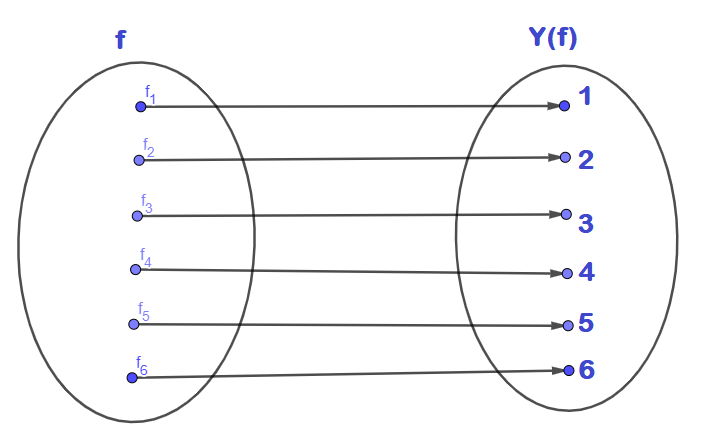
\includegraphics[scale=0.4]{figuras/va_dado.png}
	\end{figure}
 
    De forma semelhante, para a variável $X$ definida em \ref{01} temos 

        \begin{figure}[H]
            \caption{Diagrama variável $X$}
		\centering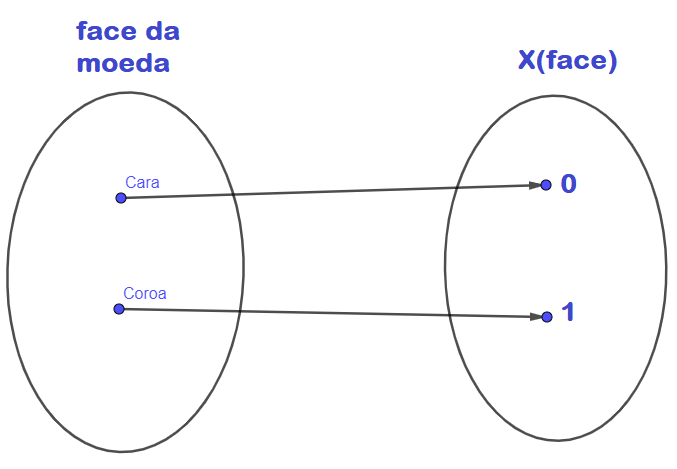
\includegraphics[scale=0.4]{figuras/va_moeda.png}
	\end{figure}

    Os dois modelos de exemplos citados são muito importantes, pois são demasiadamente citados em problemas probabilísticos e problemas de pesquisa.
    
\section{Distribuição de probabilidade}

Em linhas gerais, uma distribuição de probabilidade é uma tabela que apresenta todos os valores possíveis de uma variável aleatória juntamente com a probabilidade desses valores ocorrerem, em geral para começar a estudar bem um problema probabilístico precisamos ter bem definida a distribuição de probabilidade das variáveis em questão, por exemplo, as variáveis $X$ e $Y$ definidas anteriormente possuem as seguintes distribuições

\begin{table}[H]
        \centering
        \label{cinto}
        \begin{tabular}{c|c|c}
	    X & 0 & 1\\
	    \hline
	    $\mathbb{P}(X=x)$ & $1/2$ & $1/2$     
        \end{tabular}
    \end{table}
e 
\begin{table}[H]
    \centering
    \label{cinto}
    \begin{tabular}{c|c|c|c|c|c|c}
	Y & 1 & 2 & 3&4&5&6\\
	\hline
	$\mathbb{P}(Y=y)$ & $1/6$ & $1/6$ & $1/6$ & $1/6$ & $1/6$ & $1/6$    
    \end{tabular}
\end{table}
\inic Observe que a somas das probabilidades tem que ser sempre 1. Imagine que vamos unir esse dois jogos, então não estamos mais interessados na variáveis separada estamos por exemplo interessados em $X+Y$, como ficaria a distribuição? sendo a moeda independente do dado. 
Os possíveis valores para $Z=X+Y$ são $\{1,2,\dots,7\}$, pois podemos ter no mínimo o dado assumindo 1 e a moeda 0, bem como no máximo o dado assumindo 6 e a moeda 1, logo temos 
\begin{equation*}
    \begin{cases}
        \mathbb{P}(Z = 1) = \mathbb{P}(X=0)\mathbb{P}(Y=1) = \dfrac{1}{2}.\dfrac{1}{6} = \dfrac{1}{12}\\
        \mathbb{P}(Z = 2) = \mathbb{P}(X=0)\mathbb{P}(Y=2) + \mathbb{P}(X=1)\mathbb{P}(Y=1) = \dfrac{1}{2}.\dfrac{1}{6} + \dfrac{1}{2}.\dfrac{1}{6} = \dfrac{2}{12}\\
        \mathbb{P}(Z = 3) = \mathbb{P}(X=0)\mathbb{P}(Y=3) + \mathbb{P}(X=1)\mathbb{P}(Y=2) = \dfrac{1}{2}.\dfrac{1}{6} + \dfrac{1}{2}.\dfrac{1}{6} = \dfrac{2}{12}\\
        \vdots\\
        \mathbb{P}(Z = 6) = \mathbb{P}(X=0)\mathbb{P}(Y=6) + \mathbb{P}(X=1)\mathbb{P}(Y=5) = \dfrac{1}{2}.\dfrac{1}{6} + \dfrac{1}{2}.\dfrac{1}{6} = \dfrac{2}{12}\\
        \mathbb{P}(Z = 7) = \mathbb{P}(X=0)\mathbb{P}(Y=6) = \dfrac{1}{2}.\dfrac{1}{6} = \dfrac{1}{12}
    \end{cases}
\end{equation*}
Assim a distribuição será
\begin{table}[H]
    \centering
    \label{cinto}
    \begin{tabular}{c|c|c|c|c|c|c|c}
	Z & 1 & 2 & 3&4&5&6& 7\\
	\hline
	$\mathbb{P}(Z=z)$ & $1/12$ & $2/12$ & $2/12$ & $2/12$ & $2/12$ & $2/12$ & $1/12$    
    \end{tabular}
\end{table}
Assim, um jogo com a dinâmica da variável $Z$ os números que não são indicados apostar são $Z=1$ e $Z=7$, pois são os menos prováveis de acontecer. Podemos representar essa dinâmica via função escada.
        \begin{figure}[H]
            \caption{Diagrama variável $X$}
		\centering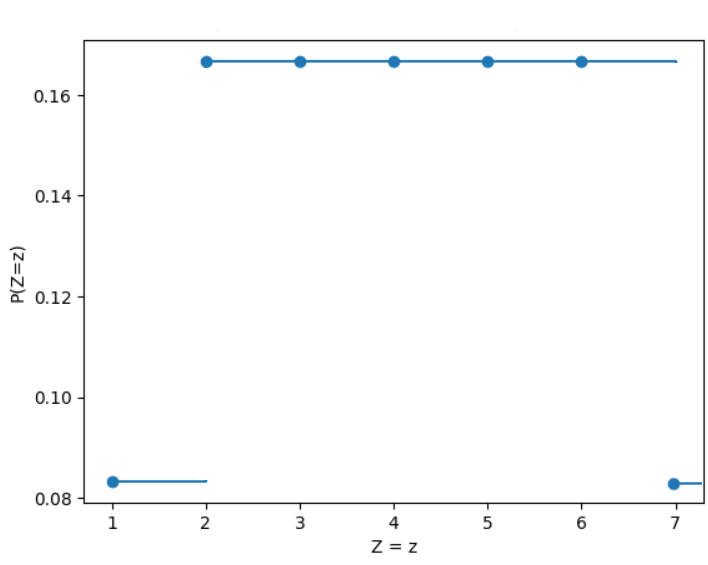
\includegraphics[scale=0.5]{figuras/va_Z.png}
	\end{figure}
    
Observe que esta estrutura de gráfico e tabelas para representar as distribuições de probabilidade não são uteis para variáveis contínuas, e para estas usaremos outra representação. 

\section{Função densidade de probabilidade}
	As funções densidade de probabilidade desempenham, no caso de variáveis aleatórias contínuas, um papel semelhante ao das funções de probabilidade no caso discreto. A principal diferença é que, para uma variável aleatória contínua, as probabilidades não são atribuídas diretamente a valores isolados, mas sim a \textbf{intervalos } do conjunto dos números reais.

Em outras palavras, se \(X\) é uma variável aleatória contínua, uma função \(f_X:\mathbb{R}\to\mathbb{R}\) será chamada de \textit{função densidade de probabilidade} de \(X\) se satisfizer as seguintes propriedades:

\begin{enumerate}
    \item[(i)] $ f_X(x)\geq 0,\qquad \forall x\in\mathbb{R},$\\
    \item[(ii)]$\int_{-\infty}^{+\infty}f_X(x),dx=1.$
\end{enumerate}

A probabilidade de \(X\) assumir um valor em determinado intervalo é obtida pela área sob a curva da função densidade nesse intervalo. Assim,

\begin{equation}
\mathbb P(a\leq X\leq b)=\int_a^b f_X(x),dx.
\end{equation}

Portanto, diferentemente do caso discreto, $f_X(x)$ não representa diretamente a probabilidade $\mathbb P(X=x)$. De fato, para uma variável aleatória contínua,

\begin{equation}
\mathbb P(X=x)=0,\qquad \forall x\in\mathbb{R}.
\end{equation}

Isso ocorre porque a probabilidade está associada à área de um intervalo, enquanto um único ponto possui comprimento nulo. Como consequência,

\begin{equation}
    \mathbb P(a<X<b)=\mathbb P(a\leq X<b)=\mathbb P(a<X\leq b)=\mathbb P(a\leq X\leq b).
\end{equation}

É importante observar ainda que a função densidade pode assumir valores maiores que \(1\). O que deve estar entre \(0\) e \(1\) é a probabilidade obtida pela integral da densidade sobre um conjunto, e não necessariamente o valor da própria função \(f_X(x)\).

\exemplo
\begin{enumerate}
    \item[(i)] A função $f(x)=-x^2$ no intervalo $[-1,1]$ não é uma função densidade, pois, para $x=1$, temos $f(1)=-1<0$, fato que por si só já elimina a possibilidade de $f$ ser uma função densidade. Além disso,
    \begin{equation}
    \int_{-1}^{1}-x^2,dx=-\left[\frac{x^3}{3}\right]_{-1}^{1}=-\left(\frac{1}{3}+\frac{1}{3}\right)=-\frac{2}{3}\neq 1.
\end{equation}
Portanto, a função viola as duas condições necessárias para ser uma função densidade de probabilidade.

\item[(ii)] Considere a função $f(x)=x+\frac{1}{2}$ no intervalo $[-1,1]$. Temos
\begin{equation}
\int_{-1}^{1}\left(x+\frac{1}{2}\right),dx
=\left[\frac{x^2}{2}+\frac{x}{2}\right]_{-1}^{1}=1.
\end{equation}
Portanto, a função satisfaz a condição de que a integral sobre todo o domínio seja igual a $1$. Entretanto, para $x=-1$, temos
\begin{equation}
f(-1)=-1+\frac{1}{2}=-\frac{1}{2}<0.
\end{equation}
Assim, $f$ não é uma função densidade, pois viola apenas a condição de não negatividade.

\item[(iii)] Considere agora a função $f(x)=x^2$ no intervalo $[-1,1]$. Como $x^2\geq0$ para todo $x\in[-1,1]$, a condição de não negatividade é satisfeita. Entretanto,
\begin{equation}
    \int_{-1}^{1}x^2\,dx
    =\left[\frac{x^3}{3}\right]_{-1}^{1}
    =\frac{2}{3}\neq1.
\end{equation}
Portanto, $f$ não é uma função densidade, pois, embora seja não negativa em todo o seu domínio, sua integral total é diferente de $1$.

\end{enumerate}

Ou seja, os exemplos (i), (ii) e (iii) mostram que nem toda função pode ser considerada uma função densidade de probabilidade. Portanto, antes de utilizarmos uma determinada função nesse contexto, devemos verificar se ela satisfaz as condições necessárias para ser classificada como uma função densidade de probabilidade.

\section{Esperança e Variância}

Até o momento, estudamos como descrever o comportamento de uma variável aleatória por meio de sua função de probabilidade, no caso discreto, ou de sua função densidade de probabilidade, no caso contínuo. Entretanto, muitas vezes estamos interessados em resumir algumas características importantes da distribuição utilizando apenas alguns valores numéricos.

Duas das medidas mais importantes para esse propósito são a \textbf{esperança} e a \textbf{variância}. De maneira intuitiva, a esperança procura indicar em torno de qual valor os possíveis resultados da variável aleatória estão distribuídos, enquanto a variância mede o quanto esses resultados tendem a se afastar desse valor.

\subsection{Esperança}

Seja $X$ uma variável aleatória. A \textbf{esperança matemática}, também chamada de \textbf{valor esperado} ou \textbf{média de $X$}, é uma medida que procura representar o valor médio da variável aleatória quando o experimento é repetido um grande número de vezes.

A esperança de $X$ será denotada por
\begin{equation}
\mathbb{E}[X]=\mu.
\end{equation}

É importante observar que $\mathbb{E}[X]$ não precisa ser um valor que a variável aleatória possa efetivamente assumir. Por exemplo, ao lançarmos um dado equilibrado, os possíveis resultados são $1,2,3,4,5$ e $6$, porém o valor esperado é $3,5$. Portanto, a esperança deve ser interpretada como uma medida de tendência central da distribuição, e não necessariamente como um possível resultado do experimento.

A maneira como calculamos $\mathbb{E}[X]$ depende do tipo da variável aleatória. Para variáveis discretas utilizamos uma soma ponderada pelas probabilidades, enquanto para variáveis contínuas utilizamos uma integral ponderada pela função densidade.

\subsubsection{Esperança de uma variável aleatória discreta}

Seja $X$ uma variável aleatória discreta que assume os valores $x_1,x_2,\ldots$ com função de probabilidade
\begin{equation}
\mathbb P(X=x_i)=p(x_i).
\end{equation}

A esperança de $X$ é definida por
\begin{equation}
    \mathbb{E}[X]=\sum_i x_i\mathbb P(X=x_i)
\end{equation}
desde que essa soma esteja bem definida.

Observe que cada possível valor $x_i$ é multiplicado pela probabilidade de sua ocorrência. Dessa forma, valores com maior probabilidade possuem maior influência sobre o valor da esperança.

Por exemplo, considere o lançamento de um dado equilibrado. Se $X$ representa o número observado na face superior, então
\begin{equation}
\mathbb P(X=x)=\frac{1}{6},\qquad x=1,2,\ldots,6.
\end{equation}
Consequentemente,
\begin{equation}
\mathbb{E}[X]=\sum_{x=1}^{6}x\mathbb P(X=x)=\frac{1}{6}(1+2+3+4+5+6)=\frac{21}{6}=3,5.
\end{equation}

Note que $3,5$ não é um possível resultado do lançamento de um dado. Esse valor representa o comportamento médio dos resultados quando imaginamos a repetição do experimento muitas vezes.

\subsubsection{Esperança de uma variável aleatória contínua}

No caso de uma variável aleatória contínua, não podemos calcular a esperança somando valores individuais, pois cada ponto possui probabilidade igual a zero. Nesse caso, utilizamos a função densidade de probabilidade.

Seja $X$ uma variável aleatória contínua com função densidade $f_X(x)$. A esperança de $X$ definida no espaço $\Theta$ é definida por
\begin{equation}
\mathbb{E}[X]
=\int_\Theta x f_X(x),dx,
\end{equation}
desde que a integral esteja bem definida.

A interpretação é semelhante ao caso discreto. O termo $x$ representa um possível valor da variável, enquanto $f_X(x)$ determina como a massa de probabilidade está distribuída em torno desse valor. Assim, a integral determina o centro médio da distribuição.

De maneira resumida, temos
\begin{equation}
\mathbb{E}[X] =
\begin{cases}
    \displaystyle\sum_x x\mathbb P(X=x),\,\, \text{se $X$ é discreta}\\ \displaystyle\int_{-\infty}^{+\infty}x f_X(x),dx,\,\, \text{se $X$ é contínua}.
\end{cases}
\end{equation}

\subsection{Variância}

Conhecer apenas a esperança de uma variável aleatória nem sempre é suficiente para compreender seu comportamento. Duas variáveis aleatórias podem possuir exatamente a mesma esperança e, ainda assim, apresentar comportamentos bastante diferentes.

Considere, por exemplo, duas variáveis aleatórias cujos valores estão concentrados em torno de sua média. Em outra situação, os valores podem estar muito espalhados, embora a média permaneça a mesma. Surge então a necessidade de uma medida capaz de quantificar essa dispersão.

A \textit{variância} de uma variável aleatória $X$ mede, em média, o quadrado da distância entre os valores de $X$ e sua esperança. Se então definimos
\begin{equation*}
    Var(X) =\mathbb{E}\left[(X-\mathbb{E}[X])^2\right].
\end{equation*}

\begin{figure}[h!]
    \centering
    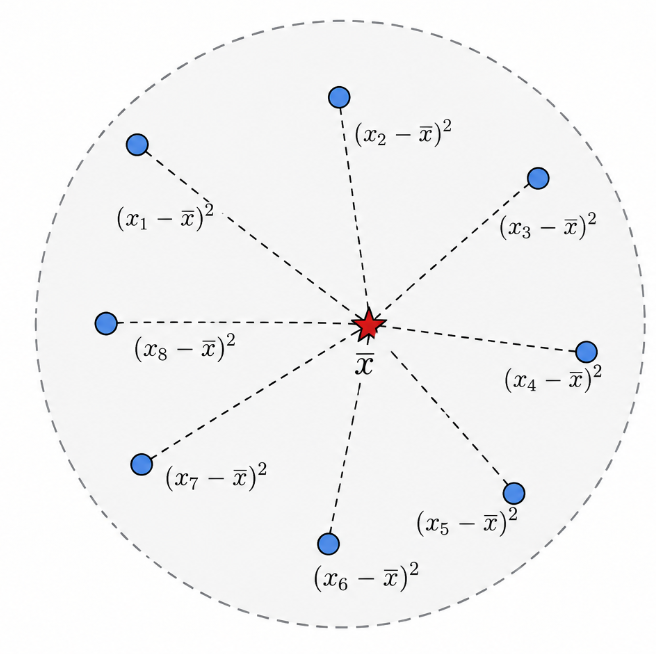
\includegraphics[width=0.7\textwidth]{figuras/variancia.png}
    \caption{Representação geométrica da variância como a média dos quadrados das distâncias das observações em relação à média.}
    \label{fig:variancia}
\end{figure}

O termo $X-\mu$ representa o desvio de $X$ em relação à sua média. Entretanto, simplesmente calcular a média desses desvios não seria útil, pois desvios positivos e negativos poderiam se cancelar. Por esse motivo, consideramos o quadrado dos desvios.

Como
\begin{equation*}
    (X-\mu)^2\geq0,
\end{equation*}
temos necessariamente
\begin{equation*}
    \operatorname{Var}(X)\geq0.
\end{equation*}

Quanto menor a variância, mais concentrados tendem a estar os valores de $X$ em torno de sua esperança. Quanto maior a variância, maior tende a ser a dispersão desses valores.

Uma forma bastante útil para o cálculo da variância é
\begin{equation*}
    \operatorname{Var}(X) =\mathbb{E}[X^2]-\left(\mathbb{E}[X]\right)^2.
\end{equation*}

Essa expressão é equivalente à definição anterior e, em muitos problemas, simplifica consideravelmente os cálculos.


\begin{defin}
    Se $X$ é uma variável aleatória discreta com função de probabilidade $p(x)=\mathbb P(X=x)$ e média $\mu=\mathbb{E}[X]$, então
\begin{equation*}
    \operatorname{Var}(X)=\sum_x (x-\mu)^2\mathbb P(X=x).
\end{equation*}

Equivalentemente, podemos utilizar
\begin{equation}
    \operatorname{Var}(X) =\sum_x x^2\mathbb P(X=x)-\mu^2.
\end{equation}

\end{defin}

Portanto, para calcular a variância de uma variável aleatória discreta, podemos primeiramente determinar $\mathbb{E}[X]$ e $\mathbb{E}[X^2]$ e, posteriormente, utilizar
\begin{equation}
\operatorname{Var}(X) =\mathbb{E}[X^2]-\left(\mathbb{E}[X]\right)^2\,\,\footnote{Esta expressão vale tanto para caso discreto quanto contínuo, mudando assim apenas a forma com que se calcula as esperanças}
\end{equation}

Se $X$ é uma variável aleatória contínua com função densidade $f_X(x)$ e média $\mu=\mathbb{E}[X]$, então
\begin{equation*}
    \operatorname{Var}(X) =\int_{-\infty}^{+\infty}(x-\mu)^2f_X(x),dx.
\end{equation*}

\begin{equation*}
    \mathbb{E}[X^2] =\int_{-\infty}^{+\infty}x^2f_X(x),dx.
\end{equation*}

Assim, embora as expressões utilizadas nos casos discreto e contínuo sejam diferentes, a ideia por trás da variância é exatamente a mesma: medir o grau de dispersão dos possíveis valores da variável aleatória em torno de sua esperança.

De maneira resumida,
\begin{equation*}
\operatorname{Var}(X)
=\begin{cases}
\displaystyle\sum_x (x-\mu)^2\mathbb P(X=x), & \text{se $X$ é discreta},\\
\displaystyle\int_{-\infty}^{+\infty}(x-\mu)^2f_X(x),dx, & \text{se $X$ é contínua}.
\end{cases}
\end{equation*}

\section{Correlação entre Variáveis}

A correlação é uma medida utilizada para quantificar a intensidade e a direção da relação linear entre duas variáveis aleatórias. Antes de defini-la formalmente, é conveniente introduzir a \textbf{covariância}. Sejam $X$ e $Y$ duas variáveis aleatórias com esperanças finitas. A covariância entre $X$ e $Y$ é definida por
\begin{equation}
\label{correlacao}
    \operatorname{Cov}(X,Y)=\mathbb{E}\left[(X-\mathbb{E}[X])(Y-\mathbb{E}[Y])\right].
\end{equation}

Equivalentemente, podemos escrever a equação~\ref{correlacao} como 

$$\operatorname{Cov}(X,Y)=\mathbb{E}[XY]-\mathbb{E}[X]\mathbb{E}[Y]\quad \footnote{Essa expressão deriva do desenvolvimento dos produtos dentro da definição e utilização de propriedades de esperança. }$$ 

    Intuitivamente, a covariância indica como $X$ e $Y$ tendem a variar conjuntamente. Quando $\operatorname{Cov}(X,Y)>0$, valores de $X$ acima de sua média tendem a estar associados a valores de $Y$ também acima de sua média. Quando $\operatorname{Cov}(X,Y)<0$, ocorre o comportamento oposto: valores elevados de uma variável tendem a estar associados a valores menores da outra.

Entretanto, a magnitude da covariância depende das unidades de medida de $X$ e $Y$, dificultando a comparação entre diferentes pares de variáveis. Para eliminar essa dependência de escala, utilizamos o \textbf{coeficiente de correlação de Pearson}, definido, para $\operatorname{Var}(X)>0$ e $\operatorname{Var}(Y)>0$, por
\begin{equation}
    \rho_{X,Y}=\frac{\operatorname{Cov}(X,Y)}{\sqrt{\operatorname{Var}(X)\operatorname{Var}(Y)}}.
\end{equation}

O coeficiente de correlação satisfaz $-1\leq\rho_{X,Y}\leq1$. Valores de $\rho_{X,Y}$ próximos de $1$ indicam uma forte associação linear positiva, enquanto valores próximos de $-1$ indicam uma forte associação linear negativa. Por outro lado, valores próximos de zero indicam ausência, ou baixa intensidade, de uma relação \textbf{linear} entre as variáveis.

\begin{figure}[h]
    \centering
    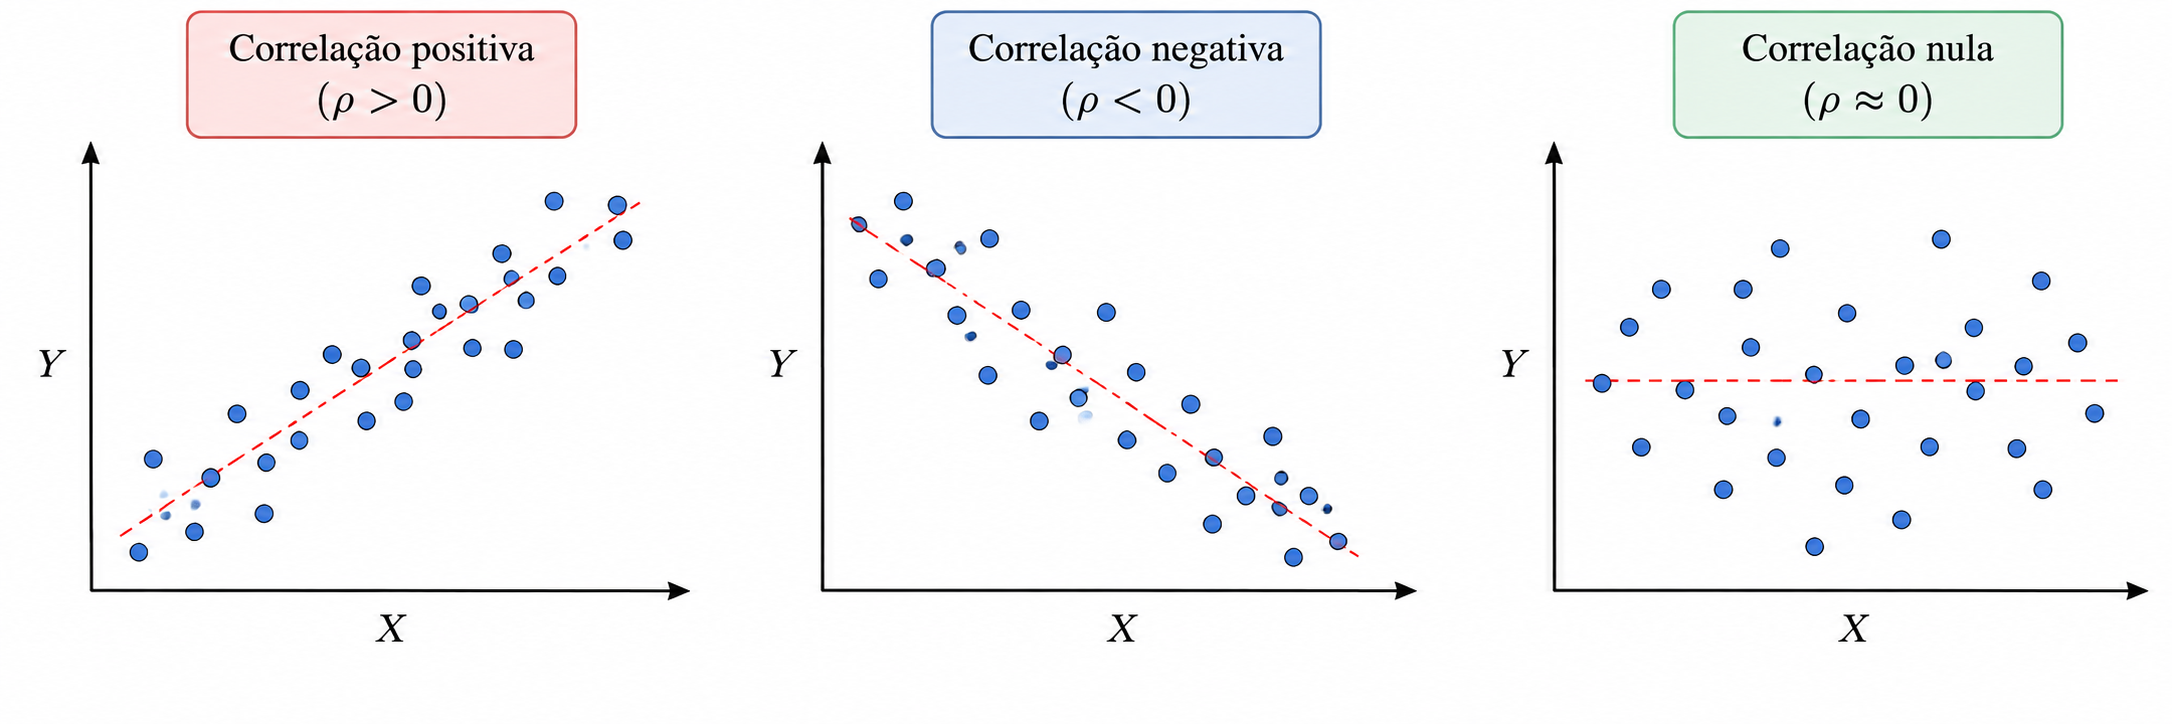
\includegraphics[width=.8\textwidth]{figuras/correlacao.png}
    \caption{Representação gráfica de diferentes padrões de correlação entre duas variáveis aleatórias $X$ e $Y$: correlação positiva, correlação negativa e ausência de correlação linear.}
    \label{fig:correlacao}
\end{figure}

É importante destacar que $\rho_{X,Y}=0$ não significa, em geral, que $X$ e $Y$ sejam independentes. Variáveis podem possuir uma forte relação não linear e, ainda assim, apresentar correlação igual a zero. Por outro lado, se $X$ e $Y$ são independentes e possuem segundos momentos finitos, então $\operatorname{Cov}(X,Y)=0$ e, consequentemente, $\rho_{X,Y}=0$, desde que ambas possuam variâncias positivas. Portanto, a correlação deve ser interpretada especificamente como uma medida de \textbf{associação linear}, e não como uma medida geral de dependência entre variáveis aleatórias.

\exercicios

    \item Considere uma sequência de lançamentos independentes de uma moeda honesta e de um dado honesto. Para $i=1,\ldots,N$, defina
\begin{equation*}
    X_i=
    \begin{cases}
        1, & \text{se a moeda resultar em cara},\\
        0, & \text{se a moeda resultar em coroa},
    \end{cases}
    \qquad
    Y_i=
    \begin{cases}
        -1, & \text{se o resultado do dado for par},\\
        1, & \text{se o resultado do dado for ímpar}.
    \end{cases}
\end{equation*}
Suponha ainda que os lançamentos da moeda e do dado sejam independentes e, para $m\leq N$, considere a variável aleatória
\begin{equation*}
    Z^{(m)}=\sum_{i=1}^{m}X_iY_i.
\end{equation*}
\begin{enumerate}
    \item[(a)] Determine a distribuição de $Z^{(m)}$.
    \item[(b)] Calcule $\mathbb E\left[Z^{(m)}\right]$ e $\operatorname{Var}\left(Z^{(m)}\right)$.
    \item[(c)] Determine $\mathbb P\left(Z^{(m)}=0\right)$ em função de $m$.
\end{enumerate}

\fimexercicios







 

 
	
	
	
	
	